\section{Floating Platform}
The floating platform, which is clearly depicted in figure \ref{fig:floatingPlatform} is the main piece of the vehicle that has been built. It's basically a baffle of gluglam wood that has two pieces of XPS cell foam as pontoons which all other components are attached to. It can keep a mass of around 20kg above water with some margins. In the middle of the floating platform two symmetrical holes with fittings has been made in which the RBR modules can be attached or detached from. In the front of the floating platform a large rounded front bumper helps with deflection of head on collisions and adds a distance between the platform and any side obstacles, which helps with maneuvering in tight spots. The back the propulsion devices has been attached, and they cannot easily be detached. In the middle of the floating platform the majority of the electronics has been placed, including the batteries. The electronics and the RBR modules also have acrylic protection covers, protecting the equipment from small splashes of water and rain.
\begin{figure}[h]
   \centering
   
\includegraphics[width=.75\textwidth]{platformWithNotes.eps}
   \caption{The floating platform without the RBR modules installed}
   \label{fig:floatingPlatform}
\end{figure}           

\subsection{RBR module}
The RBR module consists of two baffles, separated by three adjustable threaded rods. The upper mounted baffle has a modified hand-held screwdriver attached on it, which is used to attach and drive a RBR with a shaft. The lower mounted baffle a PTFE shaft guide for a RBR axle. The lower mounted baffle also has an additional baffle that goes down into the water just above where a mounted RBR will be. This is so that no large vortices will be created above the RBR. 

The upper baffle can be adjusted hight wise in order to problem dial in the depth in which a RBR will work. Usually it's enough if the RBR are on the a depth so it just passes the pontoons of the floating platform.

The speed of the RBRs can be controlled remotly through the radio controller from a low speed to up about 600 rpm on its maximum setting. Around 500 rpm is ideal, then the RBR can do its work well at the same time as the battery drain is as small as possible. 

To attach the module to the platform, it is positioned in one of the the intended slots and attached with four fly nuts and wired up to the main power supply described in the electronics section.

\subsection{Propulsion}
The propulsion is made from air-propellers installed in a acrylic plastic protection housing. In order to be able to turn, rudders have been installed in front of the propellers. These are controlled through a single servo in the back of the floating platform. The layout of the propulsion mechanism is depicted in figure \ref{fig:propellerWithNotes}. Due to the material it has been made out of the propulsion mechanism can be delicate, so care when transporting is advised. 
\begin{figure}[h]
   \centering
   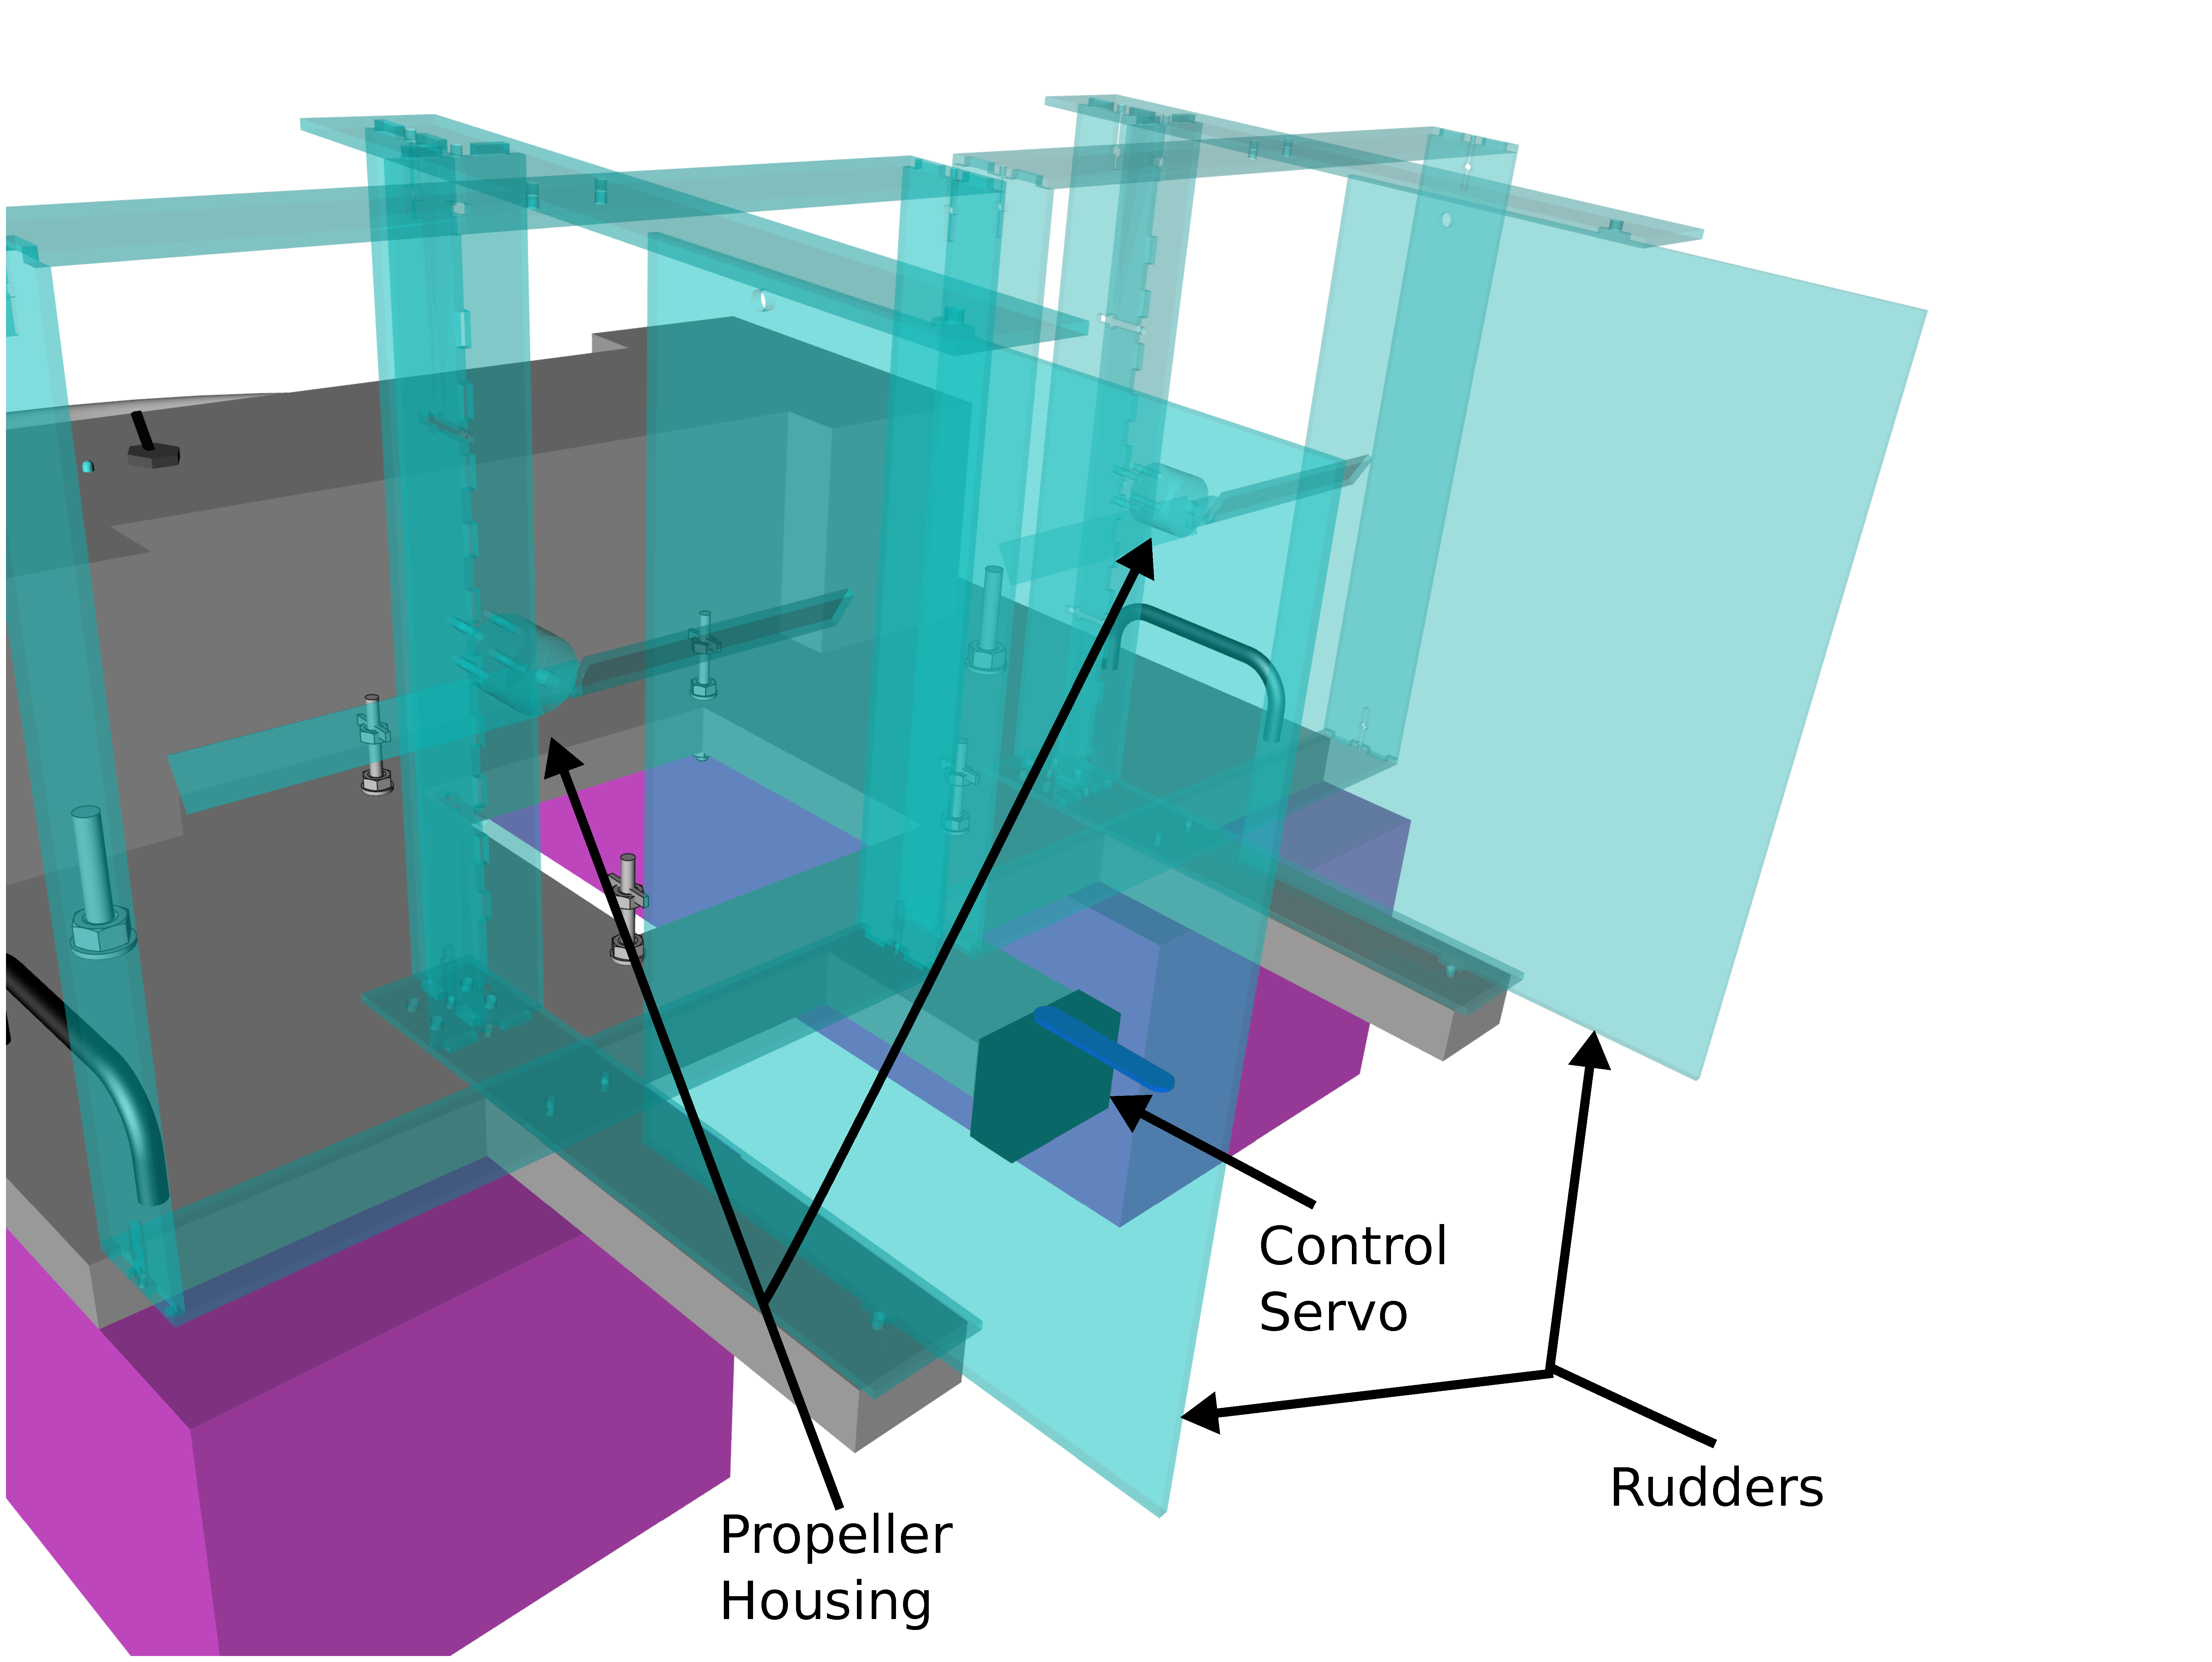
\includegraphics[width=.75\textwidth]{propellerWithNotes}
   \caption{The propulsion construction}
   \label{fig:propellerWithNotes}
\end{figure}

\subsection{Water protection}
To protect the RBR module drive assembly, the batteries, engine control units, and other electronic equipment, acrylic protection covers were manufactured. These does not protect the equipment from submersion, only from small splashes or rain. The covers for the RBR modules are easily just put ontop of the RBR modules when you want to install them. The covers for the electronics are held in place with one screw on either side of the electronic enclosure

\subsection{Transportation}
To ease transportation, the weight of the platform can be decreased by first removing the power cables from the batteries, and RBR modules, both situated underneath the protective covers. The batteries and RBR modules can then be removed by releasing the battery straps and module fly nuts which allows for removing these components. Care needs to be taken such that the propulsion mounts are not damaged during transport, as these parts are fragile.

